\documentclass[sigconf,review,anonymous]{acmart}

\AtBeginDocument{%
  \providecommand\BibTeX{{Bib\TeX}}%
}

% Review-mode metadata. Replace these fields when the FSE call for papers
% publishes the exact venue metadata for your submission cycle.
\setcopyright{none}
\settopmatter{printacmref=false}
\acmConference[FSE 'XX]
  {ACM International Conference on the Foundations of Software Engineering}
  {Month DD--DD, 20XX}
  {City, Country}

\usepackage{booktabs}
\usepackage{tabularx}
\usepackage{multirow}
\usepackage[table]{xcolor}
\usepackage{graphicx}
\usepackage{microtype}

\title{Risk-Guided Scenario Amplification for Automated Driving System Testing}

\author{Anonymous Author(s)}
\affiliation{%
  \institution{Anonymous Institution}
  \country{Anonymous}
}

\begin{document}

\begin{abstract}
Scenario-based testing is essential for evaluating autonomous driving systems (ADS), but safety-critical test generation must search a large space in which useful starting points are rare. We present a risk-guided scenario amplification framework that screens executed traffic scenarios with interaction-specific threat metrics, extracts near-miss events as optimization seeds, and perturbs the principal other vehicle within a temporally scoped window. An evolutionary search evaluates candidates against recorded ego-vehicle trajectories, avoiding repeated simulator calls during optimization, before diversity-aware selection constructs the final test suite. The current study screens 854 successfully executed SCTrans scenarios, identifies 562 threat-triggering scenarios and 731 risky interaction events, and generates 300 adversarial scenarios across ten NHTSA-derived pre-crash typologies. Closed-loop evaluation with Apollo and CARLA Traffic Manager exposes substantially different failure profiles, with lateral and non-signalized-junction conflicts producing the most severe outcomes. The results motivate risk-informed initialization as a practical direction for scalable ADS test generation.
\end{abstract}

\keywords{autonomous driving systems, scenario-based testing, risk-guided testing, evolutionary search, safety-critical systems}

\maketitle

\section{Introduction}

Autonomous driving systems (ADS), such as Apollo and Autoware, are software-intensive cyber-physical systems that integrate perception, prediction, planning, and control. Meaningful safety assurance therefore requires more than nominal-road testing: an ADS must also be exercised under rare interactions that stress assumptions shared across these software components.

Scenario-based simulation offers a reproducible way to conduct such testing, yet its effectiveness depends on which scenarios enter the generation process. Naturalistic datasets contain many realistic executions but comparatively few safety-critical interactions. Conversely, search-based generators can explore large parameter spaces, but their effectiveness and cost depend strongly on the quality of the initial seeds. Existing work has largely emphasized how to mutate or optimize a scenario; the question of which executed interactions provide promising optimization starting points remains less developed.

We investigate risk-guided scenario amplification. Starting from SCTrans scenarios~\cite{dai_sctrans_2024}, we execute each baseline with Apollo and monitor threat metrics selected according to the dominant interaction kinematics. These metrics identify near-miss ego--vehicle events and the time windows in which risk emerges. We then parameterize the principal other vehicle (POV) and use evolutionary search to amplify each interaction toward a more critical state. Candidate evaluation is performed against the recorded ego trajectory within the scoped window, which avoids a simulator call for every search iteration; selected candidates are subsequently evaluated in closed-loop simulation.

The study covers ten two-vehicle pre-crash typologies derived from the NHTSA classification~\cite{noauthor_pre-crash_nodate}. From 854 successfully executed baseline scenarios, the screening stage identifies 562 scenarios containing 731 threat-triggering events. The generation stage produces 100 candidates per typology and retains 30 diverse representatives, yielding 300 adversarial scenarios. We evaluate the resulting tests on Apollo and CARLA Traffic Manager and report changes in threat severity, collisions, and mission-level failures.

This paper makes the following contributions:

\begin{enumerate}
  \item \textbf{Risk-guided seed identification.} We use interaction-aware threat metrics to identify optimization-effective near-miss events from an executed scenario corpus.
  \item \textbf{Temporally scoped scenario amplification.} We parameterize POV behaviour only around the observed threat window and apply open-loop evolutionary optimization to reduce simulator cost.
  \item \textbf{A multi-typology empirical study.} We evaluate 300 generated scenarios spanning longitudinal, junction, and lateral conflicts on two ADS with different architectures.
\end{enumerate}

The remainder of the paper introduces the scenario and safety foundations, positions the work against related generation techniques, describes the approach, and reports the experimental results and their implications.

\section{Background}

In this Section, we provide background on existing scenario datasets and the ScTrans dataset that we use as the baseline in our adversarial generation process. We also briefly discuss the CARLA simulation platform and the two ADS used in our approach and evaluation. Then, we introduce the NHTSA pre-crash typology that categorises vehicle movements and interactions immediately prior to a crash. Finally, we discuss the thresholds that we use to classify scenarios as safety-critical based on the Euro NCAP Assisted Driving Protocol. 
\subsection{Scenario Datasets for testing ADS}\label{sec:scenario_based_testing}

Simulation-based testing has become the dominant paradigm for ADS evaluation, supported by naturalistic driving datasets such as inD~\cite{bock_ind_2020}, highD~\cite{krajewski_highd_2018}, rounD~\cite{krajewski_round_2020}, Waymo Open Dataset~\cite{sun_scalability_2020}, and nuScenes~\cite{caesar_nuscenes_2020}, as well as the CARLA Leaderboard~\cite{noauthor_carla_nodate} benchmark derived from the NHTSA pre-crash typology. We use the SCTrans dataset~\cite{dai_sctrans_2024} as the basis for our seed scenario identification. SCTrans constructs over 1,900 simulation scenarios by transforming naturalistic traffic recordings into OpenSCENARIO files compatible with CARLA and LGSVL, and demonstrates that its scenarios can boost the collision-finding capability of existing ADS fuzzers by approximately seven times. However, a fundamental limitation shared by all these datasets is that they model \textit{well-behaved} traffic participants whose actions conform to expected driving norms, leaving adversarial edge cases underrepresented.

\subsection{Simulation Platform and ADS Under Test}\label{sec:platform_ads}

We use the CARLA simulator~\cite{dosovitskiy_carla_2017}, an open-source driving platform built on Unreal Engine that provides high-fidelity rendering, realistic vehicle physics, and flexible sensor models. It supports the OpenSCENARIO and OpenDRIVE standards for reproducible scenario execution and has been widely adopted in ADS testing research~\cite{kim_drivefuzz_2022, yan_-demand_2025, li_av-fuzzer_2020}. Two ADS are evaluated:

\textbf{Apollo}~\cite{noauthor_apollo_nodate} is an open-source, industrial-grade L4 ADS integrating perception (LiDAR and camera fusion), prediction, planning, and control into a full-stack, machine-learning-based pipeline. It has been extensively used as a test subject in ADS research~\cite{dai_sctrans_2024, kim_drivefuzz_2022, yan_-demand_2025} due to its full-stack architecture and real-world deployment.

\textbf{CARLA Traffic Manager (TM)}~\cite{dosovitskiy_carla_2017} is the built-in rule-based autopilot that controls vehicle behaviour through parameterizable rules governing target speed, following distance, lane-change probability, and traffic light compliance. We include it to compare the robustness of fundamentally different ADS architectures --- one machine-learning-based and one rule-based --- against identical adversarial scenarios.

We use 854 successfully simulated scenarios from the SCTrans dataset~\cite{dai_sctrans_2024} as the starting point for our adversarial generation pipeline. SCTrans formalises the conversion from naturalistic traffic recordings to OpenSCENARIO files as a Model Transformation Problem, producing over 1,900 diverse scenarios compatible with CARLA and LGSVL. We screen these in CARLA with Apollo to identify seed scenarios that trigger our target threat metrics.

\subsection{NHTSA Pre-Crash Scenario Typology}\label{sec:NHTSA}

To ensure that the adversarial behaviours we generate reflect real-world collision patterns rather than arbitrary attack strategies, we ground our typology selection in the NHTSA Pre-Crash Scenario Typology for Crash Avoidance Research~\cite{noauthor_pre-crash_nodate}. This typology, widely adopted across the ADS community --- including by the CARLA Leaderboard~\cite{noauthor_carla_nodate} --- defines 37 pre-crash scenarios based on vehicle movements and critical events immediately prior to a crash, covering approximately 5.9 million police-reported light-vehicle crashes. We select ten two-vehicle typologies from this framework, grouped into three kinematic categories --- longitudinal, junction, and lateral --- that together account for approximately 71\% of all two-vehicle crashes. The selection criteria and category assignments are detailed in Sec.~\ref{sec:typology_selection}.

\subsection{Euro NCAP Assisted Driving Protocol}\label{sec:euro_ncap}

Having identified \textit{what} adversarial behaviours to generate, we require physically grounded thresholds to define \textit{when} a scenario becomes safety-critical. We derive these from the Euro NCAP Assisted Driving Highway \& Interurban Test and Assessment Protocol v2.2~\cite{noauthor_euro_nodate}, which specifies standardized test configurations for ACC, AEB, and Lane Support Systems across multiple collision types. The protocol's precisely specified vehicle speeds, following distances, and performance criteria provide an empirical basis for our two-tier threshold structure (critical and emergency) across five threat metrics. The specific threshold values and their derivations from the protocol are presented in Sec.~\ref{sec:threshold_selection} and Table~\ref{tab:thresholds}.
\section{Related Work}

A growing body of work targets safety-critical scenarios through adversarial methods, broadly spanning three categories. Across all categories, however, existing approaches share key limitations: scenarios are short in duration (typically $\leq5$ seconds), narrow in scope (e.g., simple junctions or single-lane interactions), and weakly grounded in realistic, complex vehicle behaviours that lead to real-world collisions.

Reinforcement learning approaches train adversarial agents to challenge the ego vehicle (e.g., Learning-to-Collide~\cite{ding_learning_2020}, D2RL~\cite{feng_dense_2023}, CRASH~\cite{kulkarni_crash_2024}, AuthSim~\cite{yang_authsim_2025}). While effective at inducing failures, they are typically confined to narrow scenario classes, require significant training cost, and often produce behaviours that lack realism or kinematic interpretability, limiting alignment with established crash typologies.

Trajectory perturbation approaches directly modify actor trajectories (e.g., AdvSim~\cite{wang_advsim_2023}, STRIVE~\cite{rempe_generating_2022}, DiffScene~\cite{xu_diffscene_2025}, CausalAF~\cite{ding_causalaf_2023}, game-theoretic methods~\cite{lin_scenario-based_2025}). Although they enable diverse scenario generation, they are generally restricted to simplified environments or pairwise interactions and do not provide systematic coverage of pre-crash scenarios.

LLM and foundation model approaches (e.g., ChatScene~\cite{zhang_chatscene_2024}, ScenGE~\cite{liu_adversarial_2025}, retrieval-augmented methods~\cite{mei_seeking_2025} , SafeBench~\cite{xu_safebench_2022}) improve diversity and plausibility through knowledge grounding. However, they still inherit limitations in scenario duration, interaction complexity, and systematic coverage of real-world pre-crash typologies.
\section{Approach}
\label{sec:approach}

This section presents our methodology for systematically generating adversarial scenarios to evaluate autonomous driving systems. Our approach has the following workflow: Sec.~\ref{sec:typology_selection} selects and justifies ten target pre-crash typologies from the NHTSA classification, grouped into three kinematic categories. Sec.~\ref{sec:threshold_selection} then establishes a two-tier threat metric framework, with threshold values derived from Euro~NCAP protocols, that provides the quantitative criteria for identifying seed scenarios and evaluating generated candidates. Finally, Sec.~\ref{sec:generation} details the adversarial generation pipeline itself, which transforms real-world near-miss events into analytically more critical test cases through parameterized perturbation, open-loop analytical optimisation, and diversity-driven selection.
\subsection{Target Pre-Crash Typology Selection}\label{sec:typology_selection}
\begin{figure}
    \centering
    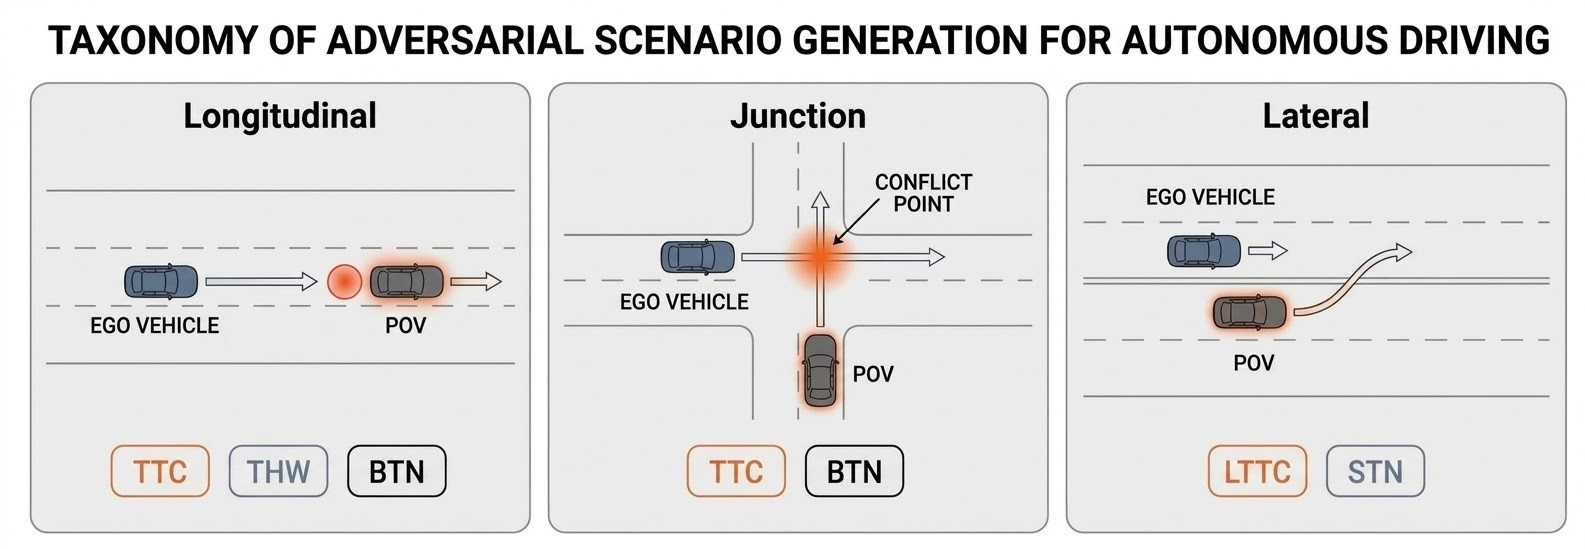
\includegraphics[width=\linewidth]{figures/scenario_taxonomy.png}
    \caption{Visual taxonomy of the three kinematic categories, their spatial configurations, associated threat metrics, and adversarial generation strategies.}

    \label{fig:scenario_taxonomy}
\end{figure}
\begin{table*}[t]
  \caption{Categorization of NHTSA Pre-Crash Scenarios and Target Threat Metrics}
  \label{tab:kinematic_categories}
  \renewcommand{\arraystretch}{1.0} 
  \begin{tabularx}{\textwidth}{@{} 
      >{\hsize=0.25\hsize\raggedright\arraybackslash}X 
      >{\hsize=0.50\hsize\raggedright\arraybackslash}X 
      >{\hsize=0.25\hsize\raggedright\arraybackslash}X 
      @{}}
    \toprule
    \textbf{Kinematic Category} & \textbf{Included Typologies (NHTSA)} & \textbf{Target Metrics} \\
    \midrule
    
    \rowcolor{blue!5}
    \textbf{Longitudinal} & 
    (1) Lead Vehicle Stopped \newline 
    (2) Lead Vehicle Decelerating \newline 
    (3) Lead Veh. Moving at Lower Speed & 
    TTC, THW, BTN \\
    
    \rowcolor{green!5}
    \textbf{Junction} & 
    (4) Veh. Turning at Non-Signalized \newline 
    (5) Straight Crossing Non-Signalized \newline 
    (6) LTAP/OD at Signalized \newline 
    (7) LTAP/OD at Non-Signalized & 
    TTC, BTN \\
    
    \rowcolor{orange!5}
    \textbf{Lateral} & 
    (8) Veh. Changing Lanes (Same Dir.) \newline 
    (9) Veh. Turning (Same Dir.) \newline
    (10) Vehicle Drifting (Same Dir.) & 
    LTTC, STN \\
    
    \bottomrule
  \end{tabularx}
\end{table*}
We select ten pre-crash typologies from the NHTSA Pre-Crash Scenario Typology for Crash Avoidance Research~\cite{noauthor_pre-crash_nodate}, drawing from two-vehicle crash scenarios ranked by frequency of occurrence. The nine highest-frequency typologies are retained directly: (1)~Lead Vehicle Stopped (20.46\%), (2)~Vehicle(s) Turning at Non-Signalized Junctions (10.83\%), (3)~Lead Vehicle Decelerating (8.96\%), (4)~Vehicle(s) Changing Lanes -- Same Direction (7.62\%), (5)~Straight Crossing Paths at Non-Signalized Junctions (6.52\%), (7)~Vehicle(s) Turning -- Same Direction (5.68\%), (8)~LTAP/OD at Signalized Junctions (5.29\%), (9)~Lead Vehicle Moving at Lower Constant Speed (4.82\%), and (10)~LTAP/OD at Non-Signalized Junctions (4.68\%). Together, these nine scenarios account for approximately 71\% of all two-vehicle light-vehicle crashes. The sixth-ranked typology, Running Red Light (6.02\%), is excluded because it constitutes an explicit traffic rule violation rather than a legitimate driving behaviour which falls outside this scope, and would be more appropriately addressed through traffic signal compliance testing rather than kinematic perturbation of the POV. In its place, we include the thirteenth-ranked typology, Vehicle(s) Drifting -- Same Direction (2.35\%), which complements the lateral kinematic category by introducing a gradual lane encroachment maneuver distinct from the abrupt lane changes captured by typology~4. This substitution ensures comprehensive coverage of lateral conflict dynamics while maintaining a physically parameterizable search space across all ten selected typologies. The ten typologies are grouped into three kinematic categories --- longitudinal, junction, and lateral --- based on the dominant conflict direction, as summarised in Table~\ref{tab:kinematic_categories} and illustrated in Fig.~\ref{fig:scenario_taxonomy}. Each category is associated with a distinct set of threat metrics that govern the objective function for scenario generation.
\begin{figure*}[t]
    \centering
    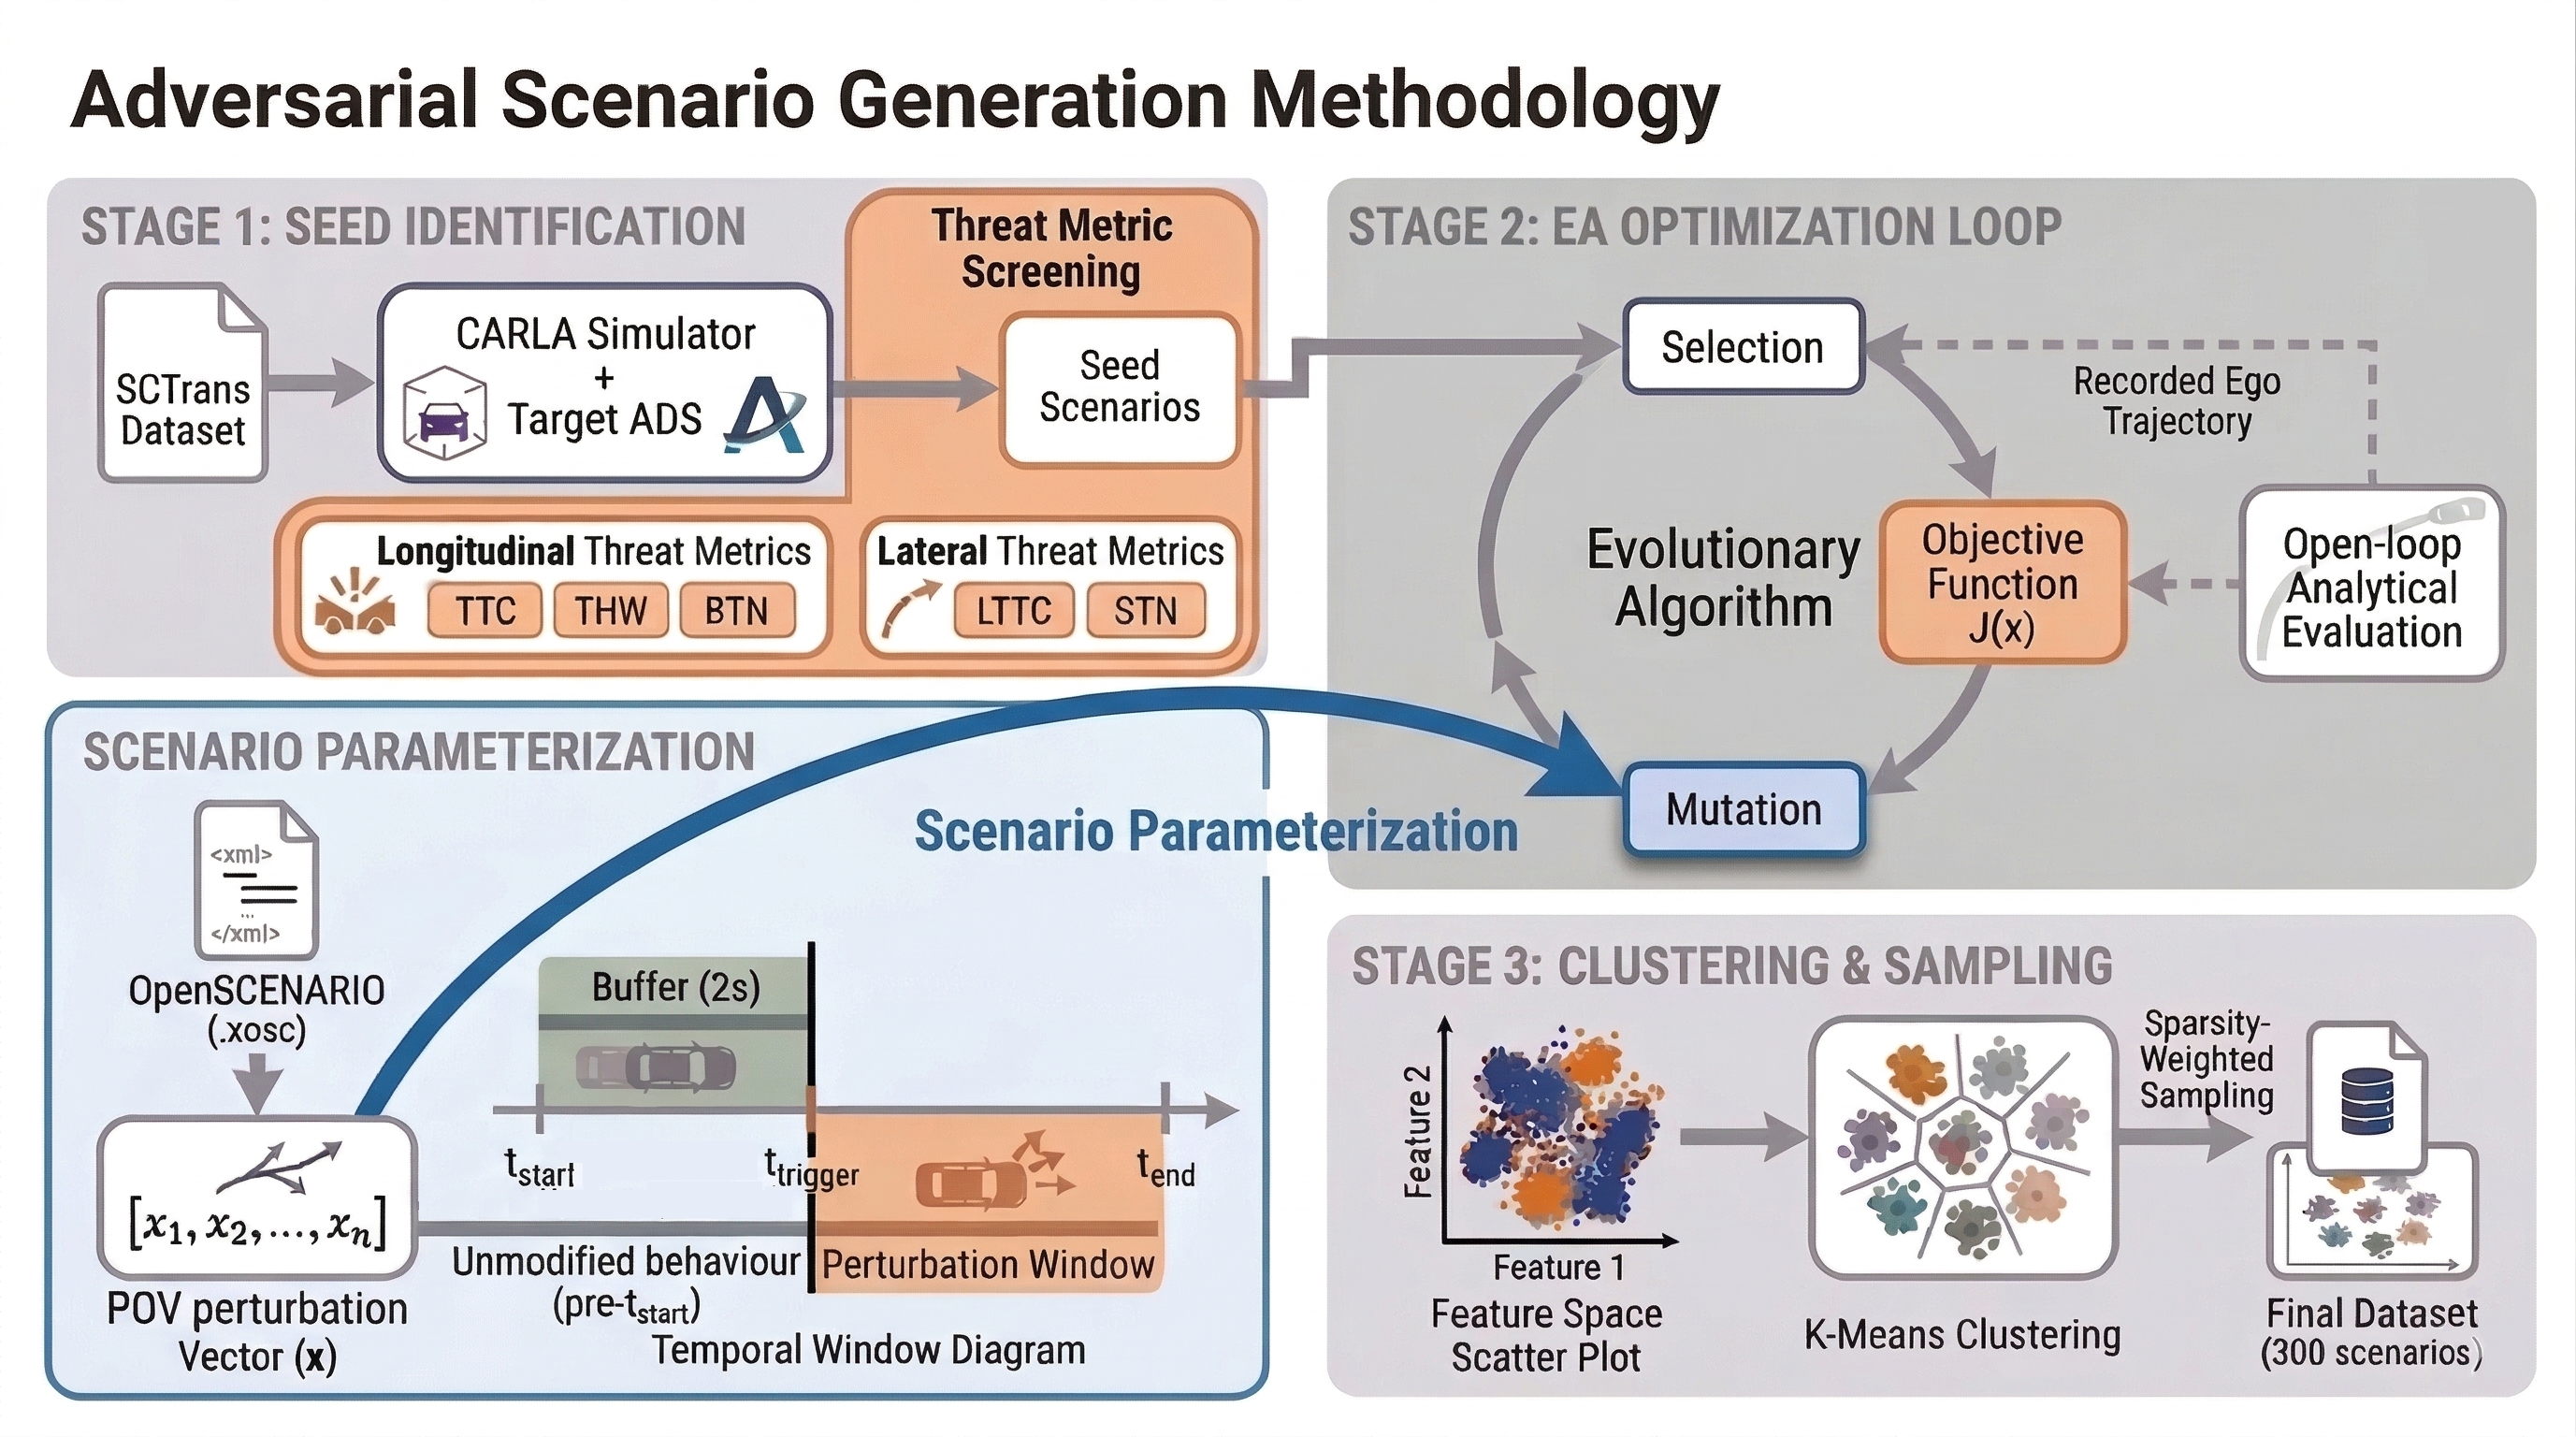
\includegraphics[width=0.8\textwidth]{figures/generation_workflow.jpg}
    \caption{Overview of the adversarial scenario generation pipeline: seed identification via threat metric screening, scenario parameterization with temporal windowing, evolutionary algorithm optimization using open-loop analytical evaluation, and diversity-driven clustering and sampling.}

    \label{fig:generation_workflow}
\end{figure*}

\subsection{Threat Metrics and Threshold Selection}
\label{sec:threshold_selection}
To identify safety-critical scenarios from the broader dataset, we require a principled method for quantifying collision risk during baseline simulations. We employ five kinematic threat metrics grouped by the dominant conflict direction. The metrics and their associated thresholds provide the quantitative foundation for both seed scenario identification and adversarial scenario evaluation.
\subsubsection{Threat Metric Definitions}
\label{sec:threat_metrics}

For longitudinal and junction conflicts, we define three metrics that capture temporal proximity and braking demand. Time-to-Collision (TTC) and Time Headway (THW) measure the temporal margin available to the ego vehicle, while the Brake Threat Number (BTN) quantifies the required deceleration relative to the vehicle's physical braking limit:
\begin{equation}
    \text{TTC} = \frac{x_{rel}}{v_{x, rel}}, \quad \text{THW} = \frac{x_{rel}}{v_{ego}}, \quad \text{BTN} = \frac{a_{x, req}}{a_{x, max}}
\end{equation}
where $x_{rel}$ and $v_{x, rel}$ are the relative longitudinal distance and velocity, $v_{ego}$ is the ego vehicle's speed, $a_{x, req}$ is the required deceleration to avoid collision, and $a_{x, max}$ is the vehicle's maximum physical braking limit. Lower TTC and THW values indicate greater temporal urgency, while higher BTN values indicate greater braking severity. To prevent mathematical instability when $v_{x, rel}$ approaches zero, the upper bounds of TTC and THW are capped at their corresponding critical thresholds as specified in Table~\ref{tab:thresholds}.

For lateral conflicts such as lane changing and drifting, $v_{x, rel}$ approaches zero, rendering TTC mathematically unstable. We therefore substitute the longitudinal metrics with Lateral Time-to-Collision (LTTC) and Steering Threat Number (STN):
\begin{equation}
    \text{LTTC} = \frac{y_{rel}}{v_{y, rel}}, \quad \text{STN} = \frac{a_{y, req}}{a_{y, max}}
\end{equation}
where $y_{rel}$ and $v_{y, rel}$ are the relative lateral distance and velocity, $a_{y, req}$ is the required lateral evasion acceleration, and $a_{y, max}$ is the maximum lateral acceleration capacity governed by road friction limits. The assignment of metrics to kinematic categories follows Table~\ref{tab:kinematic_categories}.

\subsubsection{Threshold Selection}
\label{sec:thresholds}
Each metric is assigned a two-tier threshold structure. The \textit{critical} tier identifies the onset of a safety-relevant interaction and is used to filter baseline simulations for near-miss events that serve as seed scenarios for adversarial generation. The \textit{emergency} tier defines the boundary of an unavoidable conflict and serves as the threat threshold for the optimisation process: candidate scenarios must drive at least one metric beyond its emergency threshold to be retained. The threshold values, summarised in Table~\ref{tab:thresholds}, are derived from the Euro~NCAP Assisted Driving Highway \& Interurban Test and Assessment Protocol v2.2~\cite{noauthor_euro_nodate}.

\begin{table}[htbp]
\centering
\caption{Threat metric thresholds derived from the Euro~NCAP Assisted Driving Highway \& Interurban Test and Assessment Protocol v2.2~\cite{noauthor_euro_nodate}.}
\label{tab:thresholds}
\renewcommand{\arraystretch}{1.0}
\begin{tabular}{@{}llcl@{}}
\toprule
\textbf{Metric} & \textbf{Level} & \textbf{Value} & \textbf{Derivation Basis} \\
\midrule
\multirow{2}{*}{TTC}
  & Critical  & 3.0  & ACC abort criterion (\S3.3.1.1)          \\
  & Emergency & 1.5  & FCW issuance threshold (\S4.3.1)         \\
\multirow{2}{*}{THW}
  & Critical  & 2.0  & ISO~15622 upper bound   \\
  & Emergency & 1.0  & ACC minimum gap (\S3.3.1.1)   \\
\multirow{2}{*}{BTN}
  & Critical  & 0.52 & CCRs (\S3.3.1) \\
  & Emergency & 0.80 & ACC-to-AEB transition (\S4.3.1)   \\
\multirow{2}{*}{LTTC}
  & Critical  & 1.5  & Cut-in TTC (\S3.3.1.3)   \\
  & Emergency & 0.5  & C2MC cut-in TTC (\S3.3.2.5) \\
\multirow{2}{*}{STN}
  & Critical  & 0.40 & Lane Support System (\S4.3.5) \\
  & Emergency & 0.64 & S-Bend (\S3.4.1) \\
\bottomrule
\end{tabular}
\end{table}

Of the ten threshold values, four (TTC critical and emergency, LTTC critical and emergency) are directly mapped from explicitly stated protocol parameters --- test abort criteria, warning issuance deadlines, and prescribed TTC values at lane-change completion. The remaining six are derived from the protocol's test configurations through established physical relationships: THW values from the closest following distance requirement, BTN values from the most demanding ACC scenario (CCRs) and the ACC-to-AEB transition boundary, and STN values from the LKA departure threshold and the S-Bend lateral acceleration demand.

\subsection{Adversarial Scenario Generation -- Regular Setting}\label{sec:generation}
Building on the ten target typologies and their associated threat metrics defined in Sec.~\ref{sec:typology_selection} and~\ref{sec:threshold_selection}, this section presents the adversarial scenario generation pipeline. The core objective is to transform near-miss traffic events into more critical, collision-likely test cases without violating physical plausibility. An overview of the complete pipeline is illustrated in Fig.~\ref{fig:generation_workflow}. The pipeline begins with an empirical screening phase, simulating 854 real-world traffic events from the SCTrans dataset in the CARLA simulator to identify vulnerable ``seed'' scenarios which trigger the predefined threat metrics corresponding to each typology. We frame the adversarial generation as a constrained optimization problem. By parameterizing the dynamic behavior of the Principal Other Vehicle (POV) within the OpenSCENARIO framework and constraining these bounds to Euro NCAP regulatory standards, we maintain strict kinematic realism. An evolutionary algorithm (EA) iteratively perturbs these variables using open-loop analytical evaluation against recorded ego-vehicle trajectories, guided by the typology-specific objective function. A key contribution of this methodology is the open-loop analytical optimization with temporally scoped perturbations (Sec.~\ref{sec:seed}): by restricting modifications to the threat-metric-triggered window and evaluating against recorded baseline trajectories, we achieve efficient search-space exploration while maintaining the physical validity of each generated scenario. Finally, feature-space clustering with sparsity-weighted sampling distills the results into 300 highly diverse, representative failure modes across all ten typologies.

\subsubsection{Seed Scenario Identification and Parameterization}\label{sec:seed}

The adversarial generation pipeline begins with the empirical identification of high-risk baseline events. We execute 854 original, unperturbed scenarios from the SCTrans dataset within the CARLA simulator, utilizing Apollo as the target ego vehicle. During these baseline simulations, we continuously monitor the kinematic interactions between the ego vehicle and the surrounding traffic. Scenarios that breach safe operational thresholds and trigger our target threat metrics (TTC, THW, and BTN for longitudinal conflicts; LTTC and STN for lateral conflicts) are classified as near-misses and extracted as foundational ``seed'' scenarios. The threshold values defining these near-miss boundaries are established in Sec~\ref{sec:threshold_selection}.

Once these vulnerable seeds are identified, their existing OpenSCENARIO (\texttt{.xosc}) definitions are restructured to decouple the static environment from the parameterized adversarial agent. The map topology, defined in the corresponding \texttt{.xodr} files, remains unchanged. Static environmental constraints and background non-POV traffic within the \texttt{.xosc} files are preserved, constrained to their recorded trajectories, to maintain the baseline realism of the SCTrans data. Conversely, the dynamic state of the Principal Other Vehicle (POV)---the primary adversarial agent---is parameterized to form a continuous search space. Crucially, we do not modify the entire scenario timeline. For each seed, we identify the temporal window during which the threat metrics are actively triggered, and restrict perturbations exclusively to this window plus a 2-second preceding buffer. This buffer allows the POV to transition smoothly from its unmodified baseline behavior to the perturbed, higher-risk state. All behavior prior to this window remains identical to the original scenario, ensuring that the ego vehicle's recorded trajectory up to the onset of the perturbation window is valid and unaffected.

We define a perturbation vector $\mathbf{x}$ for each seed, encompassing variables such as the POV's initial velocity ($v_{POV}$) and acceleration profiles ($a_{POV}$). We utilize OpenSCENARIO triggers, specifically the \texttt{RelativeDistanceCondition}, \texttt{RelativeSpeedCondition}, to define the exact spatial and velocity thresholds at which the POV executes risky behaviors, such as a sudden brake within a critical time window when the ego vehicle is trailing, or an aggressive lane change. By directly modifying these parameters within the \texttt{.xosc} XML structure, we create a controllable testbed ready for heuristic optimization.

\subsubsection{Defining the Objective Function}\label{sec:objective}
To guide the search algorithm toward a collision state, we formulate a fitness function $J(\mathbf{x})$ that quantitatively evaluates the danger of each candidate trajectory. The function is designed such that lower values of $J(\mathbf{x})$ indicate higher collision risk, and the evolutionary algorithm seeks to minimize it. The unified objective function is formulated as:
\begin{equation}
    J(\mathbf{x}) = \sum_{i} \mathcal{T}_{i}(\mathbf{x}) - \sum_{j} \mathcal{R}_{j}(\mathbf{x})
\end{equation}
where $\mathcal{T}_{i}(\mathbf{x})$ denotes the time-based proximity metrics (TTC/THW for longitudinal conflicts, or LTTC for lateral conflicts) and $\mathcal{R}_{j}(\mathbf{x})$ denotes the threat number metrics (BTN for longitudinal conflicts, or STN for lateral conflicts), as defined in Sec.~\ref{sec:threat_metrics}. The time-based metrics decrease as collision risk increases, while the threat numbers increase with risk; subtracting the latter ensures that all terms contribute consistently toward a lower $J(\mathbf{x})$ for higher-risk scenarios. All metrics are weighted equally, as they capture complementary aspects of collision risk: temporal margins and the required evasive effort. Minimizing $J(\mathbf{x})$ therefore simultaneously drives the scenario toward shorter time margins and greater difficulty for the ego vehicle to avoid collision.

\subsubsection{Optimization and Search Algorithm}\label{sec:optimization}
We model the generation pipeline as a constrained optimization problem, utilizing an Evolutionary Algorithm (EA) to iteratively evolve the perturbation vector $\mathbf{x}$ toward a critical collision boundary. To ensure that perturbed trajectories remain physically plausible, the allowable boundaries for $\mathbf{x}$ are strictly constrained according to the Euro NCAP AD Test and Assessment Protocol v2.2, ensuring that every generated scenario represents a standardized, kinematically valid testing condition rather than an edge-case simulator artifact. This optimization phase operates entirely through open-loop analytical evaluation rather than closed-loop simulation, enabling efficient and broad search-space exploration.

We use the ego-vehicle trajectory recorded during the preliminary baseline simulation in CARLA. For every candidate generated by the EA, we analytically superimpose the perturbed POV behavior onto this recorded trajectory. As described in Sec.~\ref{sec:seed}, perturbations are restricted to the threat-metric-triggered window and its preceding 2-second buffer, ensuring that the ego vehicle's behavior prior to this window remains identical to the baseline. By evaluating the ego vehicle in this open-loop manner---without factoring in closed-loop evasive responses---the EA is directed toward scenarios that are analytically more critical than the original seeds.

The EA employs a standard evolutionary loop: parent selection is performed across the full candidate pool, and mutation is applied to a sampled 10\% of the population at each generation to introduce controlled variation while preserving the majority of high-fitness solutions. The fitness function $J(\mathbf{x})$ evaluates the analytically superimposed trajectories using the typology-specific threat metrics to quantify the collision risk. The EA selects the parameter combinations yielding the lowest $J(\mathbf{x})$ to breed the next generation, continuously refining the POV's adversarial behavior. The EA terminates once it has collected a sufficient pool of 100 candidate scenarios that surpass at least one threat threshold for each typology. This threshold serves as a quality floor, ensuring all retained scenarios represent a meaningful increase in risk over their original seeds, while preserving diversity in the solution space for the subsequent clustering stage. The specific threat threshold values are detailed in Sec.~\ref{sec:threshold_selection} and Sec.~\ref{sec:objective}.

\subsubsection{Clustering and Selection}
Once the evolutionary algorithm produces a large pool of high-risk candidates, we distill these results into a highly diverse, non-redundant dataset. For each of the ten NHTSA typologies, the EA generates a pool of 100 candidate scenarios, each surpassing the predefined threat threshold. We then extract the kinematic features of each scenario at the point of highest threat, such as the relative speed, approach angle, and required ego-vehicle deceleration. Unlike the threat metrics used in the fitness function, which quantify pre-crash risk during optimization, these features characterize the physical crash outcome and are therefore better suited for distinguishing between structurally different failure modes. For each typology, these features are mapped into a multi-dimensional feature space and grouped using a K-Means clustering algorithm based on physical and kinetic similarity. To select the 30 representative scenarios per typology, we employ sparsity-weighted sampling: the algorithm probabilistically favors scenarios with greater distance to their nearest neighbor in feature space. This per-typology process yields a final dataset of 300 scenarios (30 $\times$ 10 typologies) that captures a wide spectrum of failure modes while avoiding redundant crash dynamics.

\section{Experimental Design}
\label{sec:experimental_design}

The revised evaluation does not primarily test the broad claim that an evolutionary algorithm can generate dangerous scenarios. Instead, it separates four questions concerning the effectiveness of risk-guided seed selection, the choice of search strategy, the transferability of the seed-selection benefit, and the comparison with gradient-based scenario generation.

\subsection{Research Questions}
\label{sec:research_questions}
%%%
\iffalse
RQ1: Comparison of our proposed method versus existing mutation-based fuzz SOTA: EA risky (E0) versus Fuzz-Random (E3)
RQ2: Comparison of our proposed method versus existing closed lopp optimization: EA risky (E0) versus King -Random (K0) 
RQ3: Performance of our approach for risky versus random seed selection : E0 versus E1
RQ4: Improvement of SOTA when using risky instead of random seed selection: King-Random (k0) versus King-Risky (K1) + Fuzz-Random (E3) versus Fuzz-Risky (E2)
\fi
%%%%

\begin{description}
    \item[RQ1:] \textbf{Does threat-guided seed selection improve evolutionary scenario generation?}
    We compare risk-triggering seeds with structurally matched ordinary interactions while keeping the evolutionary algorithm, scenario parameterization, threat objective, and search budget unchanged. This comparison isolates the contribution of seed selection (E0 vs.~E1).

    \item[RQ2:] \textbf{Does the benefit of threat-guided seed selection transfer to other search strategies?}
    We evaluate whether risky seeds also improve mutation-based fuzzing (E2 vs.~E3) and KING-native gradient-based search (K1 vs.~K0). Consistent improvements across these comparisons would suggest that the value of threat-guided seeds is not specific to a single optimizer.

    \item[RQ3:] \textbf{Does evolutionary search outperform mutation-based fuzzing under controlled conditions?}
    We compare EA and mutation-based fuzzing using identical seeds, parameter spaces, threat objectives, validity constraints, and evaluation budgets. The primary comparison uses risky seeds (E0 vs.~E2), while the comparison using random-matched seeds (E1 vs.~E3) provides supporting evidence.

    \item[RQ4:] \textbf{How does risk-guided open-loop EA compare with KING-native closed-loop optimization?}
    We compare the proposed primary configuration with KING using common closed-loop outcomes, including critical-scenario yield, collision discovery, scenario validity, diversity, simulator calls, and wall-clock cost (E0 vs.~K1, with K0 as a contextual baseline). Because the two approaches use different objectives, search spaces, and execution loops, this is an end-to-end pipeline comparison rather than a controlled comparison between EA and gradient descent.
\end{description}

\subsection{Experimental Configurations}
\label{sec:experimental_configurations}

Table~\ref{tab:experimental_configurations} summarizes the six configurations used to answer the research questions. E0 is the primary method. E0--E3 form a controlled $2\times2$ comparison of seed selection and search strategy, while K0 and K1 evaluate the effect of seed selection within KING-native optimization.

\begin{table*}[t]
    \centering
    \small
    \caption{Experimental configurations. ``Loop'' describes the search phase; candidates produced by open-loop search are subsequently evaluated through a common closed-loop validation protocol.}
    \label{tab:experimental_configurations}
    \begin{tabularx}{\textwidth}{@{}lllllX@{}}
        \toprule
        \textbf{ID} & \textbf{Seed} & \textbf{Search} & \textbf{Loop} & \textbf{Objective} & \textbf{Purpose} \\
        \midrule
        E0 & Risky & EA & Open & Threat metrics & Primary method \\
        E1 & Random-matched & EA & Open & Threat metrics & Seed-selection ablation \\
        E2 & Risky & Fuzzing & Open & Threat metrics & EA ablation \\
        E3 & Random-matched & Fuzzing & Open & Threat metrics & Seed--search interaction \\
        K0 & Random-matched & KING-Native & Closed & Collision & KING seed baseline \\
        K1 & Risky & KING-Native & Closed & Collision & Risky-seed effect on KING \\
        \bottomrule
    \end{tabularx}
\end{table*}

\subsection{Comparison Protocol}
\label{sec:comparison_protocol}

The comparisons follow five controls. First, risky and random-matched seeds are paired within the same NHTSA typology and are matched on structural properties such as road geometry, parameterizable POV behaviour, ego speed, relative distance, and interaction duration. Random-matched seeds are ordinary interactions that do not trigger the critical threat threshold. Second, E0--E3 use the same scenario representation, perturbation bounds, temporal window, threat objective, validity checks, and evaluation budget. Third, the fuzzing configurations use mutation and feedback-based corpus retention but omit population-based selection, crossover, and evolutionary reproduction. Fourth, K0 and K1 use the same KING-native action space, collision objective, closed-loop execution, and computational budget; only seed selection differs. Finally, all stochastic configurations are repeated using the same set of random seeds.

For E0--E3, open-loop search is followed by a common validation procedure. Each method searches under a fixed objective-evaluation budget, after which valid candidates crossing an emergency threshold are processed using the same diversity-selection procedure. The selected candidates are then replayed in closed-loop simulation with the target ADS. Consequently, ``open loop'' refers only to candidate search and does not imply that final outcomes are evaluated without ADS feedback.

\subsection{Hypotheses and Interpretation}
\label{sec:hypotheses}

The evaluation tests the following directional hypotheses:

\begin{itemize}
    \item \textbf{H1:} E0 outperforms E1, supporting threat-guided seed selection for EA.
    \item \textbf{H2:} E2 outperforms E3 and K1 outperforms K0, indicating that risky seeds also benefit fuzzing and KING-native search.
    \item \textbf{H3:} E0 outperforms E2 under the same risky seeds and budget, supporting EA over mutation-based fuzzing.
\end{itemize}

RQ4 is primarily comparative rather than directional. We expect E0 to require fewer simulator calls during search, whereas KING may benefit from direct closed-loop feedback and a collision-specific objective. We therefore report both effectiveness and computational cost rather than interpreting a single outcome as evidence of optimizer superiority.

The primary outcome is the number of closed-loop-confirmed critical scenarios generated under a fixed budget. Secondary outcomes include open-loop emergency-candidate yield, closed-loop confirmation rate, collision rate, risk improvement over the seed, time to first successful candidate, simulator calls, wall-clock time, scenario validity, and feature-space diversity.

\section{Results}
We present results from running the adversarial scenarios in our approach for each of the research questions in the Sections below. 

\subsection{RQ1: Impact of Adversarial Generation on Threat Severity}
\begin{table*}[t]
\centering
\caption{Mean threat metric values across 30 scenarios per typology for seed (baseline near-miss) and generated (adversarial) scenarios using Baidu Apollo. Lower TTC, THW, and LTTC indicate greater risk; higher BTN and STN reflect greater risk. Bold values breach the emergency threshold (Table~\ref{tab:thresholds}).}
\label{tab:rq1_threat_comparison}
\renewcommand{\arraystretch}{1.0}
\begin{tabular}{@{}l cc cc cc cc cc@{}}
\toprule
& \multicolumn{2}{c}{\textbf{TTC [s] $\downarrow$}} & \multicolumn{2}{c}{\textbf{THW [s] $\downarrow$}} & \multicolumn{2}{c}{\textbf{BTN [--] $\uparrow$}} & \multicolumn{2}{c}{\textbf{LTTC [s] $\downarrow$}} & \multicolumn{2}{c}{\textbf{STN [--] $\uparrow$}} \\
\cmidrule(lr){2-3} \cmidrule(lr){4-5} \cmidrule(lr){6-7} \cmidrule(lr){8-9} \cmidrule(lr){10-11}
\textbf{Typology} & Seed & Gen. & Seed & Gen. & Seed & Gen. & Seed & Gen. & Seed & Gen. \\
\midrule
\rowcolor{blue!5}
(1) Lead Veh. Stopped         & 1.60 & \textbf{1.35} & 0.80 & \textbf{0.68} & 0.781 & \textbf{0.82} & -- & -- & -- & -- \\
\rowcolor{blue!5}
(2) Lead Veh. Decelerating    & 1.80 & \textbf{1.54} & 0.90 & \textbf{0.72} & 0.617 & 0.63 & -- & -- & -- & -- \\
\rowcolor{blue!5}
(3) Lead Veh. Lower Speed     & 2.40 & \textbf{1.54} & 0.60 & 0.77* & 0.174 & 0.63 & -- & -- & -- & -- \\
\rowcolor{green!5}
(4) Turning at Non-Signalized  & 1.54 & \textbf{1.20} & -- & -- & 0.63 & 0.60 & -- & -- & -- & -- \\
\rowcolor{green!5}
(5) Straight Crossing          & 1.80 & \textbf{1.20} & -- & -- & 0.46 & 0.70 & -- & -- & -- & -- \\
\rowcolor{green!5}
(6) LTAP/OD Signalized         & 2.10 & \textbf{1.44} & -- & -- & 0.322 & 0.68 & -- & -- & -- & -- \\
\rowcolor{green!5}
(7) LTAP/OD Non-Signalized    & 1.92 & \textbf{1.20} & -- & -- & 0.43 & 0.69 & -- & -- & -- & -- \\
\rowcolor{orange!5}
(8) Changing Lanes             & -- & -- & -- & -- & -- & -- & 1.40 & \textbf{0.48} & 0.279 & 0.689 \\
\rowcolor{orange!5}
(9) Turning Same Dir.          & -- & -- & -- & -- & -- & -- & 1.50 & \textbf{0.50} & 0.126 & 0.625 \\
\rowcolor{orange!5}
(10) Drifting Same Dir.        & -- & -- & -- & -- & -- & -- & 0.73 & \textbf{0.38} & 0.320 & \textbf{1.056} \\
\bottomrule
\end{tabular}
\end{table*}

Table~\ref{tab:rq1_threat_comparison} compares mean threat metric values between seed and generated scenarios for the different adversarial typologies. We show this only for Apollo due to space constraints; the corresponding table for Traffic Manager is available in the anonymous repository.  We find that our approach is successful in consistently increasing threat severity across all ten adversarial typologies, with one exception noted below. Note that TTC, THW, and LTTC are inversely related to risk with lower values indicating a more safety-critical situation.  Whereas BTN and STN are directly proportional to risk, with higher values reflecting greater threat severity. 

\paragraph{Longitudinal Conflicts.}
TTC decreases across all three car-following typologies, most substantially in typology~3 (Lead Vehicle at Lower Speed): from 2.40\,s to 1.54\,s (36\% reduction), falling below the 1.5\,s emergency threshold. THW decreases for typologies~1 and~2, both below the 1.0\,s emergency threshold. The sole exception is typology~3, where THW increases slightly from 0.60\,s to 0.77\,s, as the EA prioritises TTC and BTN reduction when THW is already well below emergency threshold. BTN increases across all three typologies; for typology~1 it reaches 0.82, exceeding the 0.80 emergency threshold.

\paragraph{Junction Conflicts.}
All four intersection typologies show TTC reductions below 1.44\,s, with the largest in typologies~5 and~7 (both reaching 1.20\,s). BTN increases substantially, with typology~6 (LTAP/OD Signalized) showing the largest absolute increase from 0.32 to 0.68, indicating that the EA effectively tightens intersection timing to create severe braking demands.

\paragraph{Lateral Conflicts.}
The lateral typologies exhibit the most pronounced increases. LTTC drops by 48--67\% across all three typologies, with all generated values at or below the 0.5\,s emergency threshold. STN increases correspondingly; typology~10 (Drifting) reaches 1.056, exceeding 1.0 and indicating that the required lateral evasion surpasses the vehicle's physical capacity.

\paragraph{Summary.}
Our approach successfully increases threat severity across all ten adversarial typologies. Lateral conflicts are most affected, with LTTC reductions exceeding 50\% and STN approaching the vehicle's physical evasion capacity. Junction conflicts show the largest absolute BTN increases, and longitudinal conflicts exhibit consistent but more moderate degradation, with one minor exception: THW increases slightly for typology~3, as the algorithm prioritises other metrics already well below the emergency threshold.

\subsection{RQ2: Collision and Failure Outcomes}
\begin{table*}[t]
    \caption{Failure counts recorded for CARLA Traffic Manager (TM) and Baidu Apollo across kinematic scenario categories in the generated adversarial scenarios. Each cell reports the total number of failures (collisions and failure to reach destination), with the number of destination failures shown in parentheses.}
  \label{tab:collision_comparison_all}
  \renewcommand{\arraystretch}{1.0} 
  \begin{tabularx}{\textwidth}{@{} 
      >{\hsize=0.8\hsize\raggedright\arraybackslash}X 
      >{\hsize=1.6\hsize\raggedright\arraybackslash}X 
      >{\hsize=0.8\hsize\centering\arraybackslash}X 
      >{\hsize=0.8\hsize\centering\arraybackslash}X 
      @{}}
    \toprule
    \textbf{Kinematic Category} & \textbf{Typology} & \multicolumn{2}{c}{\textbf{\# collisions and undesirable behaviour}} \\
    \cmidrule(l){3-4}
    & & \textbf{TM} & \textbf{Apollo} \\
    \midrule
    \rowcolor{blue!5}
    \textbf{Longitudinal} & 
    (1) Lead Vehicle Stopped & 4(\textcolor{blue}{1}) $\uparrow$ & 1(\textcolor{blue}{1}) $\uparrow$ \\
    \rowcolor{blue!5}
     & 
    (2) Lead Vehicle Decelerating & 1 $\uparrow$ & 0 \\
    \rowcolor{blue!5}
    & (3) Lead Veh. Moving at Lower Speed & 0 & 0 \\
    \rowcolor{green!5}
    \textbf{Junction} & 
    (4) Veh. Turning at Non-Signalized & 24(\textcolor{blue}{6}) $\uparrow$ & 3(\textcolor{blue}{1}) $\uparrow$ \\
    \rowcolor{green!5}
     & 
    (5) Straight Crossing Non-Signalized & 12(\textcolor{blue}{3}) $\uparrow$ & 3 $\uparrow$ \\
    \rowcolor{green!5}
    & (6) LTAP/OD at Signalized & 17(\textcolor{blue}{2}) $\uparrow$ & 2(\textcolor{blue}{2}) $\uparrow$ \\
    \rowcolor{green!5}
    & (7) LTAP/OD at Non-Signalized & 27(\textcolor{blue}{7}) $\uparrow$ & 6(\textcolor{blue}{2}) $\uparrow$ \\
    \rowcolor{orange!5}
    \textbf{Lateral} & 
    (8) Veh. Changing Lanes (Same Dir.) & 19(\textcolor{blue}{3}) $\uparrow$ & 5(\textcolor{blue}{1}) $\uparrow$ \\
    \rowcolor{orange!5}
     & 
    (9) Veh. Turning (Same Dir.) & 14(\textcolor{blue}{7}) $\uparrow$ & 3(\textcolor{blue}{2}) $\uparrow$ \\
    \rowcolor{orange!5}
    & (10) Vehicle Drifting (Same Dir.) & 30(\textcolor{blue}{8}) $\uparrow$ & 6(\textcolor{blue}{4}) $\uparrow$ \\
    \bottomrule
  \end{tabularx}
\end{table*}

Table~\ref{tab:collision_comparison_all} presents failure counts for both ADS on the 300 adversarial scenarios. In the original SCTrans baseline, collisions occur in only 3.3\% of scenarios. The adversarial scenarios increase failure rates to 9.7\% for Apollo (29 failures) and 49.3\% for Traffic Manager (148 failures) out of total number of 300 generated scenarios.

\paragraph{Longitudinal Conflicts.}
Despite the threat increases reported in RQ1, longitudinal scenarios produce few failures: Apollo~1, TM~5 across 90 scenarios. Even typology~3, which showed the largest relative threat increase, produces zero failures for both systems. The one-dimensional nature of car-following conflicts provides a clear braking response that absorbs elevated threat levels.

\paragraph{Junction Conflicts.}
Junction scenarios show stronger correspondence between threat increases and failures: Apollo records 14 failures across 120 scenarios, TM records 80. Typology~7 (LTAP/OD Non-Signalized) produces the highest counts (TM:~27, Apollo:~6). Both systems are particularly vulnerable at non-signalized junctions, where no traffic signals regulate conflict timing and the ADS must independently predict the POV's path. Destination failures also concentrate here, suggesting that junction perturbations disrupt route planning beyond immediate collision avoidance.

\paragraph{Lateral Conflicts.}
Lateral scenarios produce the highest per-typology failure rates. Typology~10 (Drifting) triggers failures in all 30 TM scenarios and 6 Apollo scenarios. Lateral scenarios also yield the highest proportion of destination failures --- typology~10 (8/30 TM) and typology~9 (7/14 TM) --- indicating disruption to downstream path planning.

\paragraph{Summary.}
Adversarial scenarios substantially increase failure rates compared to the 3.3\% baseline, reaching 9.7\% for Apollo and 49.3\% for TM. Lateral conflicts are the most hazardous --- typology~10 (Drifting) triggers failures in all 30 TM scenarios --- followed by junction conflicts, with non-signalised junctions (typologies~4 and~7) concentrating the most failures. Longitudinal conflicts produce the most modest increase. Destination failures are disproportionately concentrated in lateral and junction scenarios, indicating that these behaviours disrupt downstream path planning beyond immediate collision avoidance.

\subsection{RQ3: ADS Robustness Comparison}

We now compare the two ADS using the results from Tables~\ref{tab:rq1_threat_comparison} and~\ref{tab:collision_comparison_all}. Overall, Traffic Manager's failure rate (49.3\%) is five times Apollo's (9.7\%), with the gap varying by kinematic category.

In \textit{longitudinal conflicts}, the difference is minimal (TM:~5, Apollo:~1), as both architectures handle one-dimensional braking effectively. In \textit{junction conflicts}, the gap widens to six-fold (TM:~80 vs Apollo:~14). Apollo's learned prediction modules provide a clear advantage in multi-directional conflicts requiring trajectory reasoning through intersections, whereas TM's fixed priority rules cannot adapt to tightened adversarial timing. Destination failures are disproportionately concentrated in TM's junction results (18 of 80). In \textit{lateral conflicts}, TM fails in 63 of 90 scenarios (70.0\%) versus Apollo's 14 (15.6\%). Typology~10 is catastrophic for TM (30/30) but Apollo is robust in the majority of cases, demonstrating that its perception pipeline can detect gradual encroachment. Typology~9 shows a distinctive pattern where 50\% of TM's failures are destination failures, indicating that lateral disruption derails path-planning even when immediate collision is avoided.

\paragraph{Summary.}
TM's rule-based architecture is consistently more vulnerable than Apollo's ML-based pipeline, with the robustness gap scaling with the dimensionality of the conflict: minimal for longitudinal braking, six-fold for multi-directional junction reasoning, and 4.5-fold for lateral evasion. Destination failures concentrate almost exclusively in TM, particularly under lateral and junction perturbations, suggesting that rule-based planning degrades not only in immediate collision avoidance but also in longer-horizon route recovery. Notably, both architectures remain vulnerable to gradual lateral encroachment and non-signalised junction conflicts, indicating that these scenario types warrant safety improvements regardless of the underlying ADS design.


\section{Discussion}

\subsection{Implications for ADS Testing}

The results suggest that safety-critical test generation benefits from separating two decisions: where search should begin and how a selected interaction should be amplified. Threat-guided screening concentrates the search on interactions that already exhibit limited safety margins, while the downstream optimizer explores feasible changes to the POV behaviour. This decomposition makes seed quality an explicit, testable component of the generation pipeline.

The strongest failures occur in lateral and non-signalized-junction conflicts. These interactions require prediction across multiple motion axes and often affect both immediate collision avoidance and longer-horizon route recovery. They therefore provide useful targets for system-level debugging spanning perception, prediction, planning, and control rather than a single component.

\subsection{Open-Loop Search and Closed-Loop Validity}

Using recorded ego trajectories avoids repeated simulator calls and enables broad exploration, but it approximates the ego vehicle's reaction to a perturbed POV. The final scenarios must therefore be replayed in closed loop, and the manuscript should explicitly report how well open-loop risk rankings predict closed-loop outcomes. Precision at the emergency threshold, rank correlation, top-$k$ retention, and simulator-call reduction would characterize this trade-off more directly.

\subsection{Threats to Validity}

\textbf{Construct validity.} Threat metrics are proxies for safety risk and may not fully capture perception errors, traffic-rule violations, passenger comfort, or responsibility for a collision. Reporting each metric and concrete outcome separately reduces, but does not eliminate, this limitation.

\textbf{Internal validity.} The current seed pool is obtained with Apollo, which may bias the selected interactions toward Apollo-specific behaviour. Simulator nondeterminism and scenario-replay variance may also affect outcomes. Repeated executions and a seed-selection comparison using matched interactions are needed for the final study.

\textbf{External validity.} The evaluation uses SCTrans, CARLA, Apollo, and TM. Results may not generalize to other datasets, simulators, maps, weather conditions, or production ADS. Replication on another corpus and ADS would strengthen the claim.

\textbf{Conclusion validity.} The existing results are descriptive. The final manuscript should use fixed search budgets, multiple random seeds, paired analyses where applicable, effect sizes, and confidence intervals.

\section{Conclusion}

We presented a risk-guided approach for amplifying near-miss traffic interactions into safety-critical ADS tests. The approach identifies promising seeds with interaction-aware threat metrics, limits perturbations to the observed threat window, applies open-loop evolutionary search, and retains a diverse set of candidates for closed-loop evaluation. Across ten NHTSA-derived typologies, the resulting scenarios expose distinct failure profiles in Apollo and CARLA Traffic Manager, with lateral and junction conflicts producing the strongest effects. These findings position seed selection as a first-class design choice for scalable scenario-based testing and motivate controlled comparisons across seed strategies, optimizers, and open- versus closed-loop evaluation.

\section{Data and Artifact Availability}

The final submission should provide an anonymous artifact containing the scenario definitions, generation implementation, configuration files, and analysis scripts. Replace this paragraph with the review-safe artifact URL and archival plan before submission.


\bibliographystyle{ACM-Reference-Format}
\bibliography{references}

\end{document}
